\documentclass[12pt]{article}

\usepackage[english]{babel}
\usepackage[a4paper,top=2cm,bottom=2cm,left=3cm,right=3cm,marginparwidth=1.75cm]{geometry}
\usepackage{listings}
\usepackage{graphicx}
\usepackage{xcolor}
\usepackage{amsmath}
\usepackage[parfill]{parskip}
\usepackage[colorlinks=true, allcolors=blue]{hyperref}

\definecolor{blue-ncs}{rgb}{0.0, 0.53, 0.74}
\definecolor{alizarin}{rgb}{0.82, 0.1, 0.26}
\definecolor{dkgreen}{rgb}{0,0.6,0}

\lstset{
    basicstyle=\ttfamily\footnotesize,
    keywordstyle=\color{blue-ncs},
    stringstyle=\color{alizarin},
    commentstyle=\color{dkgreen},
    showstringspaces=false,
    frame=single,
    breaklines=true,
}

\title{Practical 1: TCP File transfer}
\author{Truong Hoang Khanh Linh - 22BI13254}
\date{}

\begin{document}
\maketitle

\section{Protocol design}

The system is built on a simple model, including a client and a server communicating over TCP/IP.
\begin{itemize}
    \item The server acts as a file receiver and listens for client connections.
    \item The client establishs a connection to the server and sends files.
    \item Connection is done over TCP/IP connection.
\end{itemize}

Below is a sequence diagram for protocol flow:
\begin{figure}[!ht]
\centering
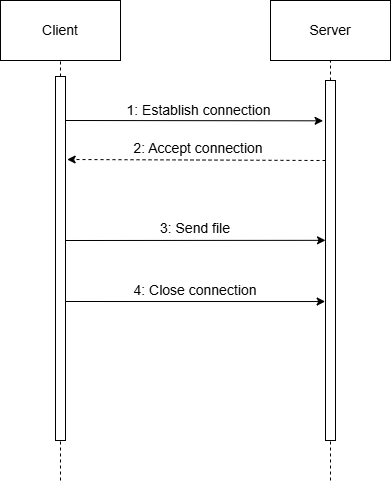
\includegraphics[scale=0.5]{protocol_design.png}
\caption{Protocol Flow}
\end{figure}


\section{System organization}

The system is organized with two oponents: a client and a server. Communication begins with the client establishing a connection to the server. The server, which is listening for incoming connections on a specified port, accepts the connection. After the connection is established, the client will send the file to the server in binary mode. The file is read in chunks of 1024 bytes and transmitted over the connection. The server receives these and write them to a file. Once the transferation is completed, the connection will be closed.

\begin{figure}[!ht]
\centering
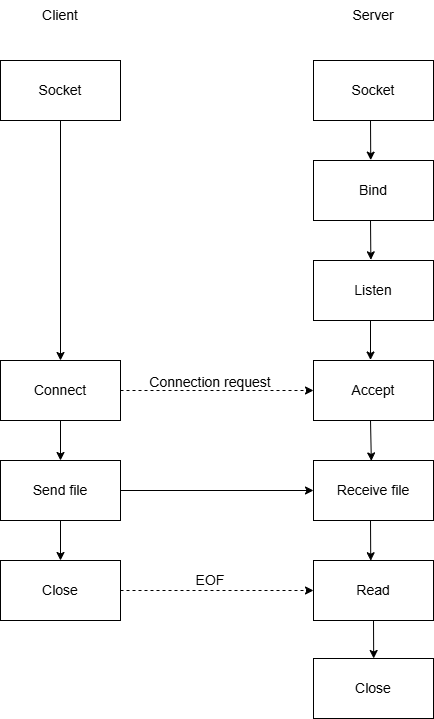
\includegraphics[scale=0.5]{system_design.png}
\caption{Sytem Architecture}
\end{figure}


\section{Implementation}
The system is implemented in Python using socket. The client and the server transfer file over TCP/IP.

\subsection{The server}
The server is binded to listen for incoming connections on a specified port using \textbf{bind()}  and \textbf{listen()}. After receiving the connection request, the server accepts the connection with \textbf{accept()} method. The sent file will be received with \textbf{recv()}.

Below is the code for the server:
\newpage
\begin{lstlisting}[language=Python]
import socket

def start_server(host='0.0.0.0', port=888):
    # Create and configure server socket
    server_socket = socket.socket(socket.AF_INET, socket.SOCK_STREAM)
    server_socket.setsockopt(socket.SOL_SOCKET, socket.SO_REUSEADDR, 1)

    server_socket.bind((host, port))

    server_socket.listen(1)
    print(f"Server listening at {host} on port {port}...")

    client_socket, client_address = server_socket.accept()
    print(f"Connection established.")

    # Receive file
    with open('received_file', 'wb') as file:
        while True:
            data = client_socket.recv(1024) 
            if not data:  # EOF
                break
            file.write(data)

    print("File received and saved as 'received_file'")
    client_socket.close()
    server_socket.close()

if __name__ == "__main__":
    start_server()
\end{lstlisting}

\subsection{The client}
The server first establishes a connection to the server using the \textbf{connect()} method. Once the server and client are connected, the client starts transmitting the file in chunks of 1024 bytes with the \textbf{send()} method. After the file is transfered successfully, the connection is closed with \textbf{close()}.

Below is the code for the client:
\newpage
\begin{lstlisting}[language=Python]
import socket

def send_file(host, port, file_path):
    # Create client socket and connect to server
    client_socket = socket.socket(socket.AF_INET, socket.SOCK_STREAM)
    
    client_socket.connect((host, port))
    print(f"Connected to server {host} on port {port}.")

    # Send file
    with open(file_path, 'rb') as file:
        while True:
            data = file.read(1024)
            if not data:
                break
            client_socket.send(data)

    client_socket.close()
    print("File sent successfully!")
    print("Connection closed.")

if __name__ == "__main__":
    send_file("192.168.86.128", 888, "transfer_file.txt")
\end{lstlisting}


\section{Testing}
First, run \textbf{server.py} to set up the server, let it listen to connections on port 888.
\begin{figure}[!ht]
\centering
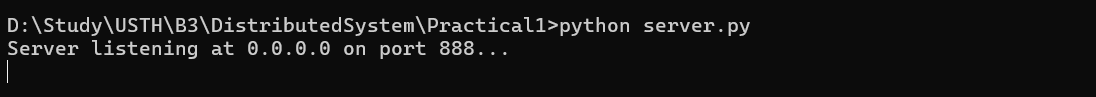
\includegraphics[scale=0.5]{test_server_1.png}
\end{figure}

After that, run \textbf{client.py} to establish the connection and transfer the file to the server. The file is now transfered successfully as shown in the images below.
\begin{figure}[!ht]
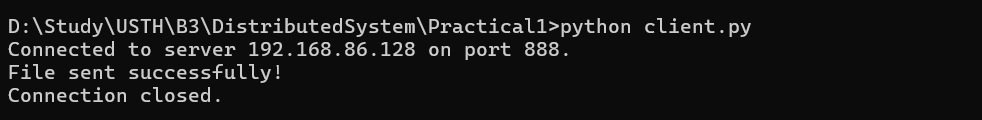
\includegraphics[scale=0.5]{test_client.png}
\end{figure}

\vspace{-0.7cm}

\begin{figure}[!ht]
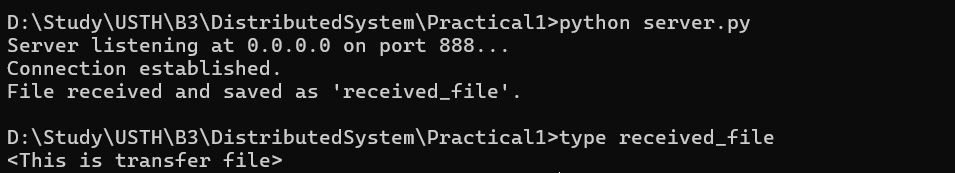
\includegraphics[scale=0.5]{test_server_2.png}
\end{figure}

\end{document}